\documentclass[sigconf,nonacm]{acmart}

\settopmatter{printacmref=false}
\setcopyright{none}
\renewcommand\footnotetextcopyrightpermission[1]{}

\usepackage{amsmath,amsfonts}
\usepackage{booktabs}
\usepackage{array}
\usepackage{graphicx}
\usepackage{mathtools}
\usepackage{xcolor}

\setlength{\textfloatsep}{6pt plus 1pt minus 2pt}
\setlength{\floatsep}{5pt plus 1pt minus 2pt}
\setlength{\intextsep}{5pt plus 1pt minus 2pt}
\setlength{\dbltextfloatsep}{6pt plus 1pt minus 2pt}
\setlength{\dblfloatsep}{5pt plus 1pt minus 2pt}
\emergencystretch=1.5em

\newcommand{\alphalife}{AlphaLife-MAS++}
\newcommand{\calA}{\mathcal{A}}
\newcommand{\calI}{\mathcal{I}}
\newcommand{\calC}{\mathcal{C}}
\newcommand{\calU}{\mathcal{U}}
\newcommand{\calM}{\mathcal{M}}
\newcommand{\calG}{\mathcal{G}}
\newcommand{\calD}{\mathcal{D}}
\newcommand{\calB}{\mathcal{B}}
\newcommand{\R}{\mathbb{R}}
\DeclareMathOperator{\argmax}{arg\,max}

\title{AlphaLife-MAS++: Auditable Cluster-Dynamic Governance for Quantitative Alpha Lifecycles}

\author{Ziyao Wang}
\affiliation{%
  \institution{Department of Mathematics and Statistics, Texas Tech University}
  \city{Lubbock}
  \state{Texas}
  \country{USA}
}
\email{ziywang@ttu.edu}

\begin{abstract}
Post-discovery alpha management is not only a return-prediction problem, but an auditable control problem over repair, deployability, redundancy, and model risk. This paper proposes AlphaLife-MAS++, a cluster-dynamic multi-agent governance system for quantitative alpha lifecycles. A Repair++ agent estimates implementation value, while liquidity, risk, challenge, and audit agents issue structured constraints and reason codes. A Governor allocates repair-risk capacity across alpha clusters using only past validation evidence and contemporaneous messages. On 153 U.S. anomaly factors from 1990 to 2024, the Cluster Dynamic Governor obtains a net Sharpe of 0.991, versus 0.943 for the Q++ repair endpoint and 0.834 for the Full MAS governance endpoint. Relative to Q++, it improves downside risk; relative to Global Dynamic, it improves stress Sharpe and expected shortfall; relative to Full MAS, it restores return while preserving most downside discipline. The gain is not driven by aggregate timing, but by cluster-level capacity allocation under proxy costs.
\end{abstract}

\keywords{quantitative finance, alpha lifecycle, multi-agent systems, offline policy learning, factor investing, auditability}

\begin{document}
\maketitle
\setlength{\bibsep}{1pt}

\section{Introduction and Related Work}

Quantitative investment research often treats alpha discovery as the central problem: a signal is proposed, backtested, and admitted into a strategy if its historical performance is strong enough. Deployment is different. A live alpha library is a dynamic collection of research assets. Signals can become redundant with other signals, load on known risk premia, move through temporary drawdowns, become capacity constrained, or decay as competition and arbitrage change market structure. The operational decision is therefore not only whether an alpha was once valid, but how much repair risk the portfolio should admit today under liquidity, redundancy, challenge, and audit constraints.

This paper studies post-discovery alpha governance as an auditable multi-agent control problem. Each alpha is represented by an Alpha Card containing rolling performance, residualized evidence, correlation, implementation history, lifecycle state, and audit fields. Specialized agents observe different parts of the card and emit typed messages: Repair++ submits implementation-value claims, Liquidity prices deployability, Risk prices redundancy and style concentration, Challenge flags overfit or placebo-sensitive actions, and Audit records the decision packet. A Governor arbitrates these messages and allocates repair-risk capacity across alpha clusters. The agent terminology is not intended to describe free-form language-model negotiation or unconstrained autonomous trading. The machine-learning object is a structured policy over alpha-month states, implementation actions, capacity budgets, and constraints.

The paper connects empirical asset pricing, alpha decay, online allocation, offline policy learning, and multi-agent governance. Asset pricing documents broad cross-sectional predictability through size, value, momentum, profitability, investment, quality, and related characteristics \cite{fama1992cross,fama1993common,jegadeesh1993returns,carhart1997persistence,novyMarx2013other,asness2013value,fama2015five,hou2015digesting}. Large anomaly libraries show both breadth and fragility \cite{green2017characteristics,feng2020taming,jensen2023replication}, while multiple-testing and data-snooping work warns against interpreting selected backtests as clean evidence \cite{white2000reality,hansen2005test,harvey2016and,bailey2014deflated}. Alpha decay and publication effects suggest that deployed signals can weaken after discovery \cite{mclean2016does}. Liquidity research shows why gross anomaly returns can diverge from implementable payoffs \cite{amihud2002illiquidity,acharya2005asset,pastor2003liquidity,frazzini2018trading}.

From the machine-learning side, formulaic alpha work shows that executable alphas can be compactly represented \cite{kakushadze2016formulaic}, and financial machine learning expands the candidate predictor set \cite{gu2020empirical}. Online portfolio selection and robust portfolio construction study sequential allocation under estimation error \cite{cover1991universal,li2014online,demiguel2009optimal,ledoit2004well}. Offline policy learning provides tools for improving policies from logged historical data \cite{dudik2011doubly,sutton2018reinforcement}. Multi-agent systems add a complementary perspective: heterogeneous agents can hold private observations, local objectives, and conflicting permissions, coordinated by blackboard or arbitration mechanisms \cite{hayesroth1985blackboard,stone2000multiagent,wooldridge2009introduction,shoham2008multiagent}. Lifecycle-state modeling also relates to structural breaks and latent regimes \cite{bai1998estimating,rabiner1989tutorial,adams2007bayesian}.

Relative to these literatures, the contribution is not a new alpha discovery engine. First, the paper formalizes post-discovery alpha management as auditable multi-agent control rather than a stock-level prediction task. Second, it introduces Repair++ as a distributional implementation-value agent embedded inside a constrained governance system. Third, it introduces the Cluster Dynamic Governor, which allocates repair-risk capacity across alpha clusters rather than applying a single global timing rule. Fourth, it shows empirically that cluster-level capacity control improves the realized risk-adjusted frontier. The main evidence is not that a global gate predicts when Q++ will beat Full MAS. That predictability is weak. The stronger evidence is that cluster-level capacity allocation improves stress Sharpe and expected shortfall relative to aggregate dynamic capacity control and centralized cluster overlays, while preserving an auditable governance endpoint.

This positioning is deliberately narrower than a standard strategy paper. The system is evaluated as a governance layer for a library of already-discovered alphas. Its objective is to decide how much repair risk should be admitted, where it should be admitted, and which objections should bind. This is close to an institutional model-risk problem: a portfolio manager may want to know not only whether an implementation switch has positive historical value, but whether that value comes from a fragile equal-weighted channel, whether it overlaps with a crowded style cluster, whether a challenge test shows placebo sensitivity, and whether the decision can be replayed after the fact. AlphaLife-MAS++ is designed around those questions.

\section{Auditable Cluster-Dynamic MAS}

Let \(\calA=\{1,\ldots,N\}\) be a library of discovered alphas and let time be monthly. For alpha \(j\) and month \(t\), \(r_{j,t}(a)\) denotes the realized return under implementation action \(a\in\calU\), where \(\calU\) includes value-weighted, equal-weighted, value-weighted-cap, residualized, liquidity-constrained, or no-repair implementations. All decisions for month \(t+1\) are functions of the information set \(\calI_t\). Future returns enter only through historical training labels, validation windows, or out-of-sample evaluation.

Each alpha has an Alpha Card \(c_{j,t}\in\calC\). Agent \(i\in\calG\) observes a private slice \(o^i_{j,t}=O_i(c_{j,t},\calD_t)\), where \(\calD_t\) is the data available at month \(t\). It writes a structured message
\begin{equation}
m^i_{j,t}=(\hat y^i_{j,t},\rho^i_t,b^i_{j,t},v^i_{j,t},\ell^i_{j,t})\in\calM ,
\end{equation}
where \(\hat y^i_{j,t}\) is a numerical claim, \(\rho^i_t\) is reliability, \(b^i_{j,t}\) is a bound or penalty, \(v^i_{j,t}\) is a veto, and \(\ell^i_{j,t}\) is a reason code. A decision packet stores the card snapshot, all messages, accepted and rejected actions, binding constraints, final weights, realized outcomes, and postmortem fields.

The Alpha Card is the shared state object that prevents the system from becoming a loose collection of verbal agent opinions. In the implementation it contains rolling Sharpe and \(t\)-statistics, 12- and 24-month returns, maximum correlation with other alphas, residualized health after FF6 adjustment, coverage, implementation history, lifecycle state, and audit hashes. The Monitoring Agent can use the performance fields, the Repair++ Agent can use counterfactual implementation returns, the Liquidity Agent can inspect coverage and equal-weighted exposure, and the Audit Agent can verify that the required fields are present. Agents therefore communicate through a common object while retaining different permissions.

The Repair++ Agent estimates implementation payoffs as a distributional claim rather than a point forecast. For action \(a\), it emits
\begin{equation}
\widehat Q^{++}(c_{j,t},a)=
(\widehat\mu_{j,t,a},\widehat q^{5}_{j,t,a},\widehat q^{50}_{j,t,a},\widehat q^{95}_{j,t,a},
\widehat p^{win}_{j,t,a},\widehat p^{tail}_{j,t,a},\widehat\sigma^{model}_{j,t,a}).
\end{equation}
The empirical estimator is a rolling ensemble of a ridge model and a histogram gradient-boosted tree, refit annually on a 180-month window with a 12-month label embargo. Features include rolling alpha health, Sharpe, \(t\)-statistics, 12- and 24-month returns, residualized health, maximum correlation, coverage, implementation-specific return and drawdown features, equal-weighted share, and blend indicators. Residual quantiles from the training window calibrate \(q^5,q^{50},q^{95}\), while ensemble dispersion produces model uncertainty. The estimator itself is not the theoretical contribution. Its role is to provide a return-seeking repair claim that must pass through liquidity, risk, challenge, and audit constraints before entering the portfolio.

The Full MAS endpoint is also rule-bound rather than discretionary. Its weights are proportional to a health score combining raw and FF6-residualized health, multiplied by lifecycle-state and regime gates. Repair-value messages can increase weights through a bounded exponential term. Liquidity, risk, and challenge messages enter as disagreement penalties, veto penalties, and risk-reason penalties; any hard veto reduces but does not automatically delete an alpha unless audit or data validity fails. The endpoint therefore represents a transparent governance policy built from typed messages, not an undisclosed optimizer tuned directly on final performance.

The main Governor is cluster dynamic. Let \(\calC_1,\ldots,\calC_K\) denote alpha clusters obtained from pre-sample residual correlation structure. The Governor chooses a repair-risk capacity
\[
b_{c,t}\in[0,1]
\]
for each cluster \(c\). A high \(b_{c,t}\) admits more Repair++ exposure in that cluster; a low \(b_{c,t}\) shifts the cluster toward governance-constrained Full MAS exposure. The Governor solves the stylized objective
\begin{equation}
\begin{aligned}
\max_{w_t,\pi_t,\{b_{c,t}\}}\quad
&\sum_{c=1}^{K}\sum_{j\in c}\sum_{a\in\calU}
w_{j,t}\pi_{j,t,a}
\left[b_{c,t}S^{repair}_{j,t,a}+(1-b_{c,t})S^{gov}_{j,t,a}\right] \\
&-\eta_t w_t^\top\Sigma_t w_t-\tau_t TO_t-\kappa_t CVaR_t-\chi_t Capacity_t .
\end{aligned}
\label{eq:cluster_gov}
\end{equation}
Here \(S^{repair}_{j,t,a}\) comes from Repair++ payoff claims, while \(S^{gov}_{j,t,a}\) comes from liquidity, redundancy, challenge, audit, veto, and risk-cap messages. The empirical implementation is an endpoint-capacity approximation to Eq.~\eqref{eq:cluster_gov}. For each cluster, the system first constructs a return-seeking Q++ sleeve and a governance-constrained Full MAS sleeve, then realizes
\[
R^{++}_{c,t+1}=b_{c,t}R^{Q++}_{c,t+1}+(1-b_{c,t})R^{gov}_{c,t+1}.
\]
This approximation keeps the implementation replayable while retaining the economic interpretation of \(b_{c,t}\) as repair-risk capacity. The cluster budget is selected using only past validation evidence:
\begin{equation}
\begin{aligned}
b_{c,t}=\argmax_{b\in\calB}\quad
&\widehat U^{val}_{c,t}(b)
-\lambda_{smooth}(b-b_{c,t-1})^2  \\
&-\lambda_{shrink}(b-b^{global}_{t})^2 .
\end{aligned}
\label{eq:budget}
\end{equation}
The shrinkage term is important. Cluster capacity expands the feasible set relative to a global budget, but it also introduces estimation risk. Shrinking local budgets toward a global budget regularizes the extra flexibility.

The global model is the restricted case \(b_{1,t}=\cdots=b_{K,t}=b_t\). Therefore, cluster capacity can add value only if repair reliability is heterogeneous across clusters. Weak aggregate timing does not imply zero cluster-allocation value: even if \(b_t\) has little predictive power for the aggregate Q++ minus Full MAS gap, cluster-level budgets can improve utility by limiting repair exposure in fragile clusters and preserving it where repair value is more stable. This is the theoretical interpretation used below. We do not claim that \(b_{c,t}\) is a precise one-month return timing signal.

This distinction is central for inference. A global timing story would require evidence that the aggregate budget \(b_t\) predicts the next realized gap between Q++ and Full MAS. The experiments do not support that strong claim. A cluster-capacity story is weaker and more realistic: the Governor regularizes a cross-section of repair exposures, so the benefit can come from reducing tail co-movement, avoiding concentration in fragile clusters, and allowing repair exposure where the validation record is less unstable. In this sense the budget is a control variable, not a forecast marketed as a signal.

\begin{figure*}[t]
  \centering
  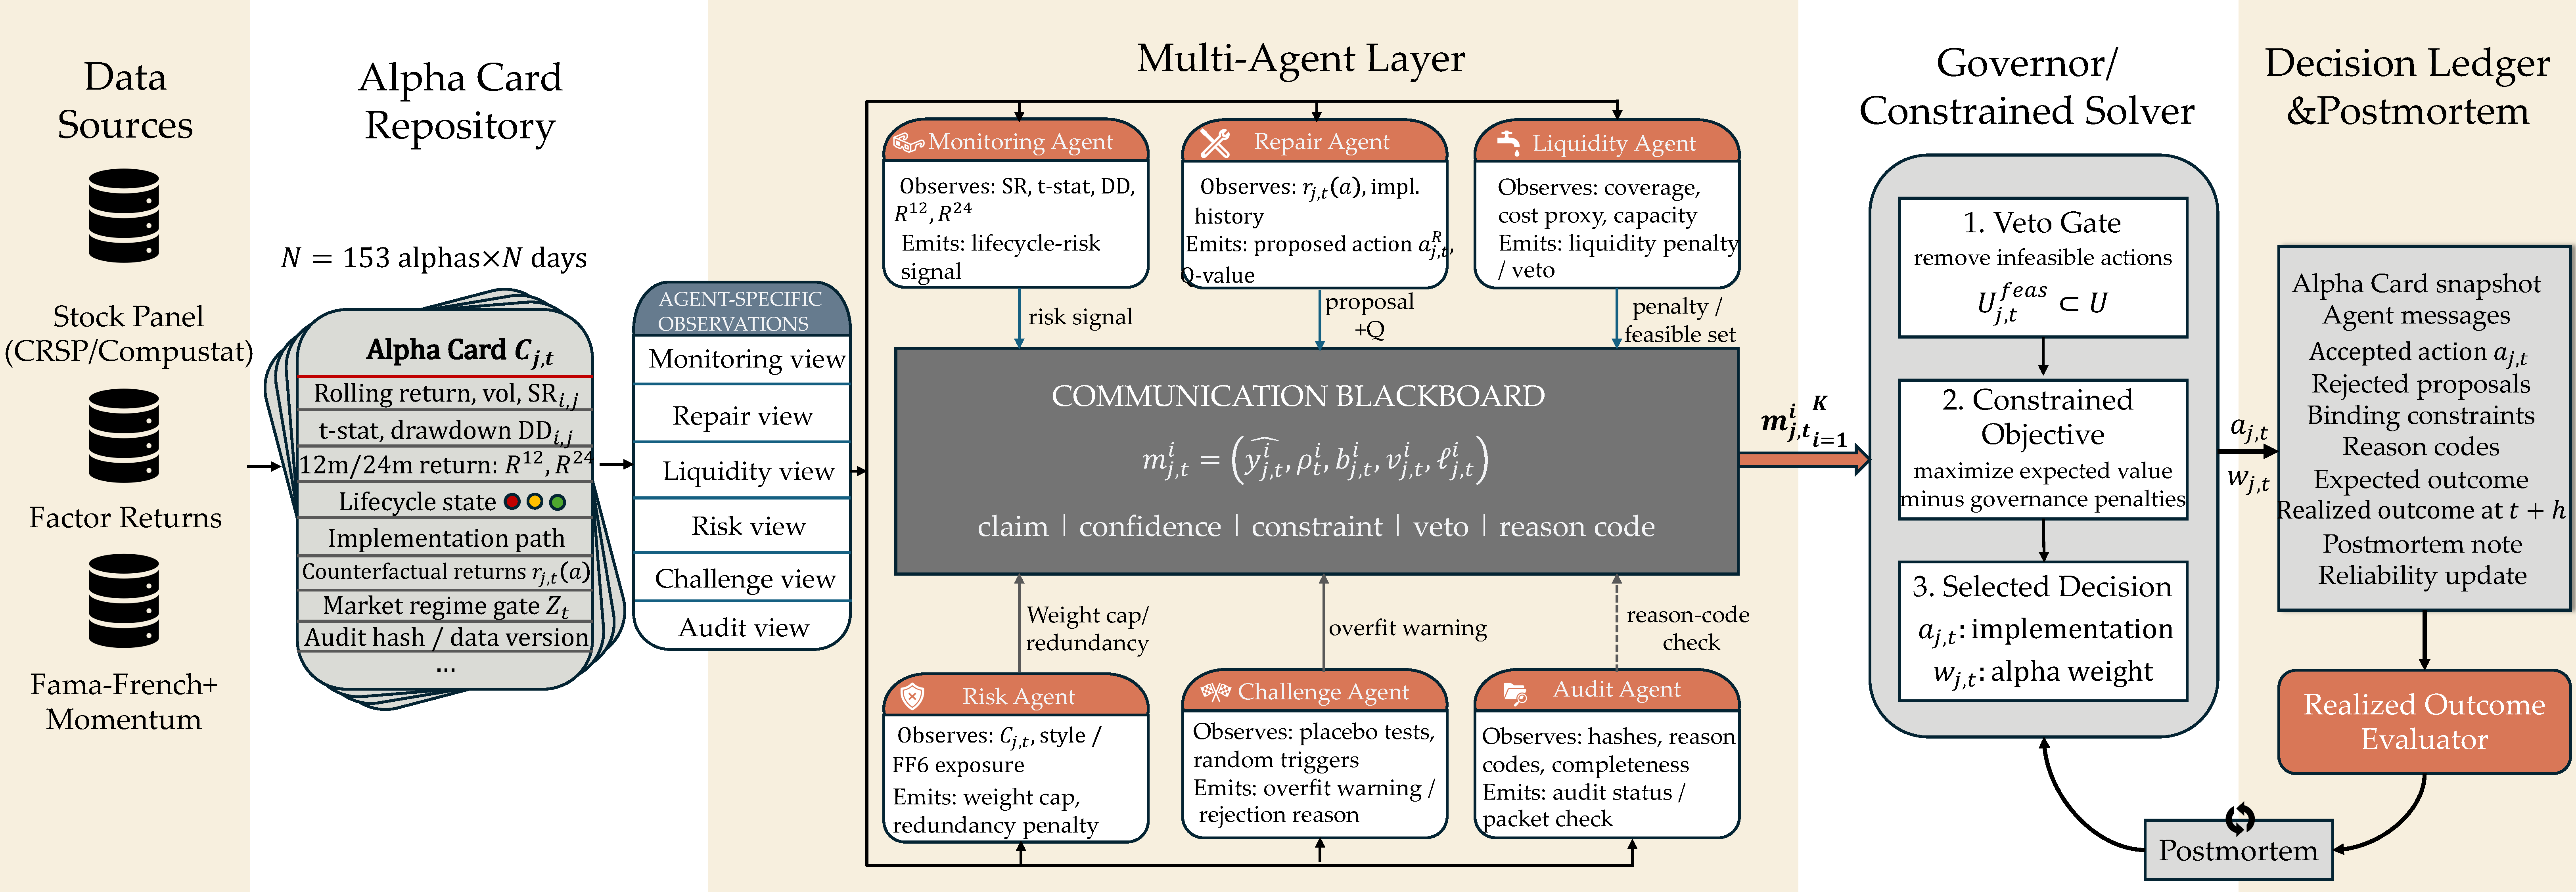
\includegraphics[width=\textwidth,height=0.31\textheight,keepaspectratio]{figures/figure1.png}
  \caption{AlphaLife-MAS++ architecture. Agents observe private slices of the Alpha Card repository, write structured proposal, critique, veto, and confidence messages to a blackboard, and a Governor solves constrained implementation, weighting, and cluster-level repair-risk capacity decisions. The decision ledger stores accepted actions, rejected proposals, constraint status, realized outcomes, and reliability updates.}
  \Description{A detailed architecture diagram of the AlphaLife-MAS++ governance system.}
  \label{fig:architecture}
\end{figure*}

\begin{table}[t]
\centering
\caption{Agent contracts in the MAS++ control system.}
\label{tab:contracts}
\scriptsize
\setlength{\tabcolsep}{2.5pt}
\begin{tabular}{p{0.19\columnwidth}p{0.31\columnwidth}p{0.31\columnwidth}}
\toprule
Agent & Private observation & Permission \\
\midrule
Monitoring & rolling performance, drawdown, state risk & lifecycle risk signal \\
Repair++ & counterfactual implementation payoffs & distributional repair claim \\
Liquidity & coverage, cost proxy, capacity proxy & shadow price or veto \\
Risk & correlation graph, style exposure & cluster cap, redundancy penalty \\
Challenge/Audit & placebo, trace completeness, reason codes & overfit warning, decision packet \\
\bottomrule
\end{tabular}
\end{table}

\begin{table}[t]
\centering
\caption{Decision packet fields used for audit replay.}
\label{tab:packet}
\scriptsize
\setlength{\tabcolsep}{2.4pt}
\begin{tabular}{p{0.28\columnwidth}p{0.58\columnwidth}}
\toprule
Field & Stored content \\
\midrule
State snapshot & Alpha Card features and data version at \(\calI_t\) \\
Agent messages & claims, confidence, constraints, vetoes, reason codes \\
Capacity decision & selected \(b_{c,t}\), validation window, shrinkage target \\
Portfolio decision & implementation map, alpha weights, binding constraints \\
Postmortem & realized returns, rejected-action outcomes, reliability update \\
\bottomrule
\end{tabular}
\end{table}

\section{Experimental Protocol}

The empirical setting is a U.S. monthly anomaly alpha library built from 153 JKP-style factor returns from 1990 to 2024. Each alpha has value-weighted, equal-weighted, and value-weighted-cap implementations. Fama-French five factors plus momentum are used for residualized diagnostics and final performance attribution \cite{fama1993common,carhart1997persistence,fama2015five}. The decision unit is an alpha-month. All policy choices use trailing information; repair labels and validation utilities are constructed with an embargo.

The main endpoints are Q++ and Full MAS. Q++ is the return-seeking Repair++ endpoint: it selects implementations from the distributional action-value model and alpha health weights. Full MAS is the governance endpoint: it applies typed vetoes, disagreement penalties, redundancy controls, and audit constraints. MAS++ capacity models allocate between these endpoints at different levels. Fixed capacity uses a constant repair-risk budget \(b\). Global dynamic capacity chooses one \(b_t\) for the whole library. Cluster Dynamic Governor chooses \(b_{c,t}\) for each alpha cluster according to Eq.~\eqref{eq:budget}. A reliability overlay adds an additional conservative shrinkage based on recent realized regret.

Clusters are formed before the final test comparison from residual alpha return correlations. The factor-return histories begin in January 1963, while evaluation begins in January 1990. Clustering uses the 1970--1989 pre-sample window only; all 153 alphas have at least 60 non-missing observations in that window, and average coverage is 99.8\%. The main specification uses eight agglomerative clusters with average-linkage distance derived from residual correlations. This number is intentionally not the best ex post choice in the robustness grid. It is a parsimonious middle specification that allows heterogeneity without giving the Governor too many degrees of freedom. The cluster budget is chosen from \(\{0.35,0.50,0.60,0.70,0.80,0.90,0.95\}\) using a 120-month validation window, a 60-month minimum history, and shrinkage toward the global budget. Thus, the cluster model expands the global model's feasible set but does not freely fit a separate timing rule for every alpha.

Baselines include the two endpoints, fixed-capacity MAS++ at several budgets, global dynamic capacity, cluster dynamic capacity, and cluster dynamic with reliability. The fixed-capacity baselines are strong: they test whether a simple static convexification of Q++ and Full MAS is already sufficient. The global dynamic baseline tests aggregate timing. Two additional centralized cluster overlays use the same cluster-budget machinery but replace the Full MAS governance endpoint with either centralized constrained Q or inverse-volatility allocation. These baselines test whether the result is only a generic cluster overlay rather than a MAS governance endpoint. The cluster dynamic baseline tests the paper's main mechanism: cross-sectional repair-risk capacity allocation under typed governance constraints.

The repair endpoint is trained in a full-information counterfactual setting. For the same alpha-month, the value-weighted, equal-weighted, value-weighted-cap, and equal-weighted/value-weighted-cap blend implementations are all observable in the historical factor library, so the Repair++ Agent can learn from counterfactual implementation outcomes rather than from only the action taken by a logged policy. The target is a multi-horizon utility combining 3-, 6-, and 12-month implementation improvement over the value-weighted baseline. The prediction layer also estimates win probability, left-tail probability, and model uncertainty; these enter the Governor as repair claims rather than as unconstrained orders.

Transaction costs are proxied because the public factor-return setting does not provide full holdings or order-book data. Net returns subtract 10 bps times alpha-library weight turnover and 2 bps times implementation switching; the stress case uses 25 bps and 5 bps; the extreme case uses 50 bps and 10 bps. These are not live execution-cost estimates. They are common implementability penalties used to compare policies under the same assumptions. Performance is reported as net Sharpe, stress Sharpe, annual net return, maximum drawdown, 5\% expected shortfall, turnover, implementation switching, and FF6 alpha \(t\)-statistics. Inference uses moving-block bootstrap intervals for Sharpe and downside differences \cite{lo2002statistics,newey1987simple}.

The empirical protocol is therefore intentionally adversarial to the main claim. If Q++ alone were sufficient, fixed or cluster governance should not improve the risk-adjusted frontier. If a static convexification were sufficient, fixed \(b=0.60\) or \(b=0.80\) would match Cluster Dynamic. If aggregate timing were the mechanism, Global Dynamic would dominate fixed capacity and the global budget would predict the Q++ minus Full MAS gap. The results below separate these possibilities.

\section{Main Results}

Table~\ref{tab:main} reports the main result. The return-seeking Q++ endpoint has the highest annual return, 4.72\%, but weaker downside performance. The governance endpoint has the strongest downside discipline, but its Sharpe is lower. Fixed-capacity MAS++ already improves the frontier, showing that repair and governance endpoints are complementary. The main specification, Cluster Dynamic Governor, performs best because it allocates repair-risk capacity across alpha clusters rather than applying a single aggregate budget.

\begin{table}[t]
\centering
\caption{Main performance. Net Sharpe uses the 10/2 bps proxy cost; stress Sharpe uses the 25/5 bps cost.}
\label{tab:main}
\scriptsize
\setlength{\tabcolsep}{2.0pt}
\resizebox{\columnwidth}{!}{%
\begin{tabular}{llrrrrrr}
\toprule
Block & Strategy & Net SR & Stress SR & Ann. ret. & Max DD & ES5 & FF6 \(t\) \\
\midrule
Return endpoint & Q++ & 0.943 & 0.893 & 4.72\% & -10.92\% & -3.32\% & 4.54 \\
Governance endpoint & Full MAS & 0.834 & 0.829 & 3.04\% & -8.51\% & -2.19\% & 5.66 \\
Fixed capacity & \(b=0.60\) & 0.957 & 0.886 & 3.95\% & -9.41\% & -2.67\% & 5.20 \\
Fixed capacity & \(b=0.80\) & 0.942 & 0.858 & 4.26\% & -9.91\% & -2.95\% & 4.73 \\
Aggregate control & Global dynamic & 0.948 & 0.863 & 4.13\% & -9.42\% & -2.83\% & 5.07 \\
Cluster control & Cluster dynamic & 0.991 & 0.910 & 3.94\% & -8.74\% & -2.58\% & 5.54 \\
Reliability overlay & Cluster reliability & 0.978 & 0.900 & 3.93\% & -8.61\% & -2.62\% & 5.35 \\
Non-MAS cluster & Central Q def. & 0.934 & 0.860 & 4.45\% & -11.99\% & -3.25\% & 4.90 \\
Non-MAS cluster & Inv-vol def. & 0.980 & 0.894 & 3.58\% & -7.53\% & -2.30\% & 4.92 \\
\bottomrule
\end{tabular}
}
\end{table}

The most important comparison is not simply Cluster Dynamic versus Full MAS. Relative to Q++, Cluster Dynamic gives up annual return but improves maximum drawdown by 2.19 percentage points and expected shortfall by 0.74 percentage points. Relative to Full MAS, it preserves most downside discipline while increasing annual return by 0.90 percentage points and raising Sharpe from 0.834 to 0.991. Relative to a fixed \(b=0.60\) budget, it improves Sharpe and stress Sharpe with similar annual return. Relative to Global Dynamic, it improves every risk-adjusted statistic in the table. The centralized cluster baselines clarify the role of the governance endpoint. Replacing Full MAS by centralized constrained Q weakens both Sharpe and downside risk. Replacing it by inverse volatility produces lower drawdown, but also lower annual return, stress Sharpe, and FF6 \(t\)-statistics. The empirical conclusion is therefore not that a global gate predicts when Q++ will outperform. It is that cluster-level capacity allocation improves the realized risk-adjusted frontier when the defensive endpoint is an auditable MAS governance policy.

\begin{table}[t]
\centering
\caption{Bootstrap inference for Cluster Dynamic Governor. Positive drawdown and ES5 differences mean the first strategy has smaller drawdown or less negative expected shortfall.}
\label{tab:boot}
\tiny
\setlength{\tabcolsep}{2.0pt}
\resizebox{\columnwidth}{!}{%
\begin{tabular}{lrrrr}
\toprule
Comparison & SR diff. & Stress SR diff. & DD diff. & ES5 diff. \\
\midrule
Cluster - Q++ & 0.048 & 0.017 & 2.19\% & 0.74\% \\
\quad bootstrap \(p\) & 0.345 & 0.750 & 0.057 & 0.000 \\
Cluster - Full MAS & 0.157 & 0.082 & -0.23\% & -0.39\% \\
\quad bootstrap \(p\) & 0.145 & 0.443 & 0.865 & 0.032 \\
Cluster - Fixed \(b=0.60\) & 0.034 & 0.025 & 0.67\% & 0.09\% \\
\quad bootstrap \(p\) & 0.271 & 0.430 & 0.142 & 0.468 \\
Cluster - Global dynamic & 0.044 & 0.048 & 0.69\% & 0.25\% \\
\quad bootstrap \(p\) & 0.052 & 0.030 & 0.120 & 0.005 \\
Cluster - Central cluster & 0.057 & 0.051 & 3.25\% & 0.66\% \\
\quad bootstrap \(p\) & 0.406 & 0.450 & 0.056 & 0.000 \\
Cluster - Inv-vol cluster & 0.011 & 0.017 & -1.21\% & -0.28\% \\
\quad bootstrap \(p\) & 0.721 & 0.594 & 0.093 & 0.000 \\
\bottomrule
\end{tabular}
}
\end{table}

Table~\ref{tab:boot} shows where the evidence is strongest. The Sharpe improvement over Q++ is not statistically significant. The downside improvements are much stronger, especially expected shortfall. The cleanest evidence for the MAS++ mechanism is Cluster Dynamic versus Global Dynamic: stress Sharpe and expected shortfall improve under cluster-level capacity control. The centralized cluster comparison also matters. Using the same cluster-budget machinery with a centralized constrained-Q defensive endpoint leaves materially worse drawdown and expected shortfall. An inverse-volatility defensive endpoint is safer in absolute downside terms, but it does not match the main model's stress Sharpe. These comparisons keep the interpretation narrow: Cluster Dynamic is not a universal minimum-risk allocation, but it improves the risk-adjusted frontier relative to aggregate timing and non-MAS cluster overlays.

The reliability overlay is informative but not the main model. It reduces maximum drawdown from -8.74\% to -8.61\%, but it lowers Sharpe from 0.991 to 0.978 and stress Sharpe from 0.910 to 0.900. We therefore treat reliability as a conservative governance overlay rather than as the performance driver. A more selective reliability model, conditioned on reason codes and cluster-specific regret, is a natural extension, but the current evidence supports the simpler Cluster Dynamic Governor as the main specification.

\begin{table}[t]
\centering
\caption{Mechanism diagnostics. Buckets are cluster-months sorted by \(b_{c,t}\). Return gaps are monthly; volatility and ES5 are computed over the bucket sample.}
\label{tab:mechanism}
\scriptsize
\setlength{\tabcolsep}{2.5pt}
\resizebox{\columnwidth}{!}{%
\begin{tabular}{lrrr}
\toprule
Diagnostic & Low budget & Medium budget & High budget \\
\midrule
Average \(b_{c,t}\) & 42.7\% & 66.6\% & 85.2\% \\
Q++ minus Gov return gap & 0.047\% & -0.006\% & 0.061\% \\
Q++ volatility & 2.53\% & 2.40\% & 1.37\% \\
Q++ ES5 & -5.97\% & -4.68\% & -2.76\% \\
Q++ return in Q++ tail months & -1.93\% & -0.27\% & -0.37\% \\
\bottomrule
\end{tabular}
}
\end{table}

Table~\ref{tab:mechanism} is deliberately included because it narrows the interpretation. The cluster budgets are not a precise one-month return-timing signal. A global-budget regression for the next-month Q++--Full MAS gap has slope \(0.0002\) with \(t=0.09\). A cluster fixed-effect regression has slope \(0.0028\) with \(t=1.22\), and low-, medium-, and high-budget groups are not monotone in realized return gaps. The more appropriate interpretation is portfolio-level capacity control. High-budget clusters have much lower Q++ volatility and less severe Q++ expected shortfall than low-budget clusters. The Governor therefore uses past validation evidence to regularize how much repair risk enters each cluster, limiting exposure where repair is historically fragile and preserving repair where it is more stable.

Budget dispersion is also economically meaningful. The average Cluster Dynamic repair budget is 64.7\%, while the average active repair weight is 62.4\%. This places the policy between the return endpoint and the governance endpoint rather than collapsing to either extreme. Across the eight clusters, average budgets range from 53.7\% to 72.4\%, and the cross-cluster budget standard deviation averages about 9.1\%. Higher-budget clusters include investment/accounting-quality variables and seasonality variables; lower-budget clusters include broad value/size/beta and profitability/mispricing groups. The model is therefore not making a single market-timing decision; it is reallocating the repair-risk channel across economically related groups of alphas.

\section{Robustness and Subperiods}

The Cluster Dynamic result is not driven by a single shrinkage parameter. Table~\ref{tab:robust} varies the shrinkage parameter in Eq.~\eqref{eq:budget}. The main value, \(\lambda=20\), is not the Sharpe-maximizing value; it is a middle specification. Results remain above 0.97 Sharpe even under much stronger shrinkage. The result is also stable across cluster counts. The main specification uses eight clusters for parsimony, while ten and twelve clusters are slightly stronger in-sample. We retain eight clusters to avoid selecting the largest reported Sharpe.

\begin{table}[t]
\centering
\caption{Robustness to shrinkage and cluster count. Main specification uses eight clusters and \(\lambda=20\).}
\label{tab:robust}
\scriptsize
\setlength{\tabcolsep}{2.8pt}
\begin{tabular}{lrrrr}
\toprule
Specification & Net SR & Stress SR & Max DD & ES5 \\
\midrule
\(\lambda=5\) & 0.997 & 0.919 & -8.45\% & -2.52\% \\
\(\lambda=10\) & 0.997 & 0.917 & -8.57\% & -2.54\% \\
\(\lambda=20\) main & 0.991 & 0.910 & -8.74\% & -2.58\% \\
\(\lambda=40\) & 0.981 & 0.899 & -8.93\% & -2.64\% \\
\(\lambda=80\) & 0.970 & 0.887 & -9.11\% & -2.70\% \\
\midrule
6 clusters & 0.959 & 0.883 & -9.00\% & -2.63\% \\
8 clusters main & 0.991 & 0.910 & -8.74\% & -2.58\% \\
10 clusters & 0.996 & 0.915 & -8.72\% & -2.58\% \\
12 clusters & 0.994 & 0.913 & -8.76\% & -2.58\% \\
\bottomrule
\end{tabular}
\end{table}

Subperiod results in Table~\ref{tab:subperiod} further limit the claim. Cluster Dynamic is not uniformly the highest-Sharpe policy in every period. In 2005--2014, Q++ remains stronger, which means governance capacity sometimes sacrifices upside in repair-friendly regimes. In 2020--2024, absolute Sharpe remains low, but Cluster Dynamic improves on both endpoints. The system's contribution is therefore not uniform return dominance. It delivers the best full-sample risk-adjusted frontier while reducing the severity of weak-regime outcomes.

The 2005--2014 period is the most important failure case. Q++ has Sharpe 0.657, while Cluster Dynamic has 0.596. This does not contradict the governance claim: in some regimes, the repair endpoint earns more by carrying fragile exposure that the Governor partially suppresses. Conversely, in 2020--2024, Q++ Sharpe falls to 0.173 and Cluster Dynamic rises to 0.275, slightly above Full MAS. The policy is therefore better understood as a risk-frontier allocator than as a uniformly dominant timing model.

\begin{table}[t]
\centering
\caption{Subperiod Sharpe ratios.}
\label{tab:subperiod}
\scriptsize
\setlength{\tabcolsep}{3.0pt}
\begin{tabular}{lrrrr}
\toprule
Strategy & 1990--2004 & 2005--2014 & 2015--2024 & 2020--2024 \\
\midrule
Q++ & 1.292 & 0.657 & 0.585 & 0.173 \\
Full MAS & 1.293 & 0.479 & 0.307 & 0.256 \\
Fixed \(b=0.60\) & 1.375 & 0.596 & 0.517 & 0.198 \\
Global dynamic & 1.341 & 0.577 & 0.580 & 0.196 \\
Cluster dynamic & 1.418 & 0.596 & 0.585 & 0.275 \\
Cluster reliability & 1.394 & 0.604 & 0.570 & 0.281 \\
\bottomrule
\end{tabular}
\end{table}

\section{Auditability, Deployment, and Limits}

Auditability is a first-class output. For every monthly decision, the system records Alpha Card snapshots, data versions, agent messages, conflicts, rejected actions, final implementation maps, final weights, cluster budgets, constraint status, realized outcomes, and postmortem fields. This matters because a failed repair can be caused by structural signal decay, liquidity pressure, redundancy, or an unlucky but defensible decision. A replayable packet does not make the decision correct, but it makes the reasoning falsifiable.

The design also limits language-model use. A language model can summarize a decision packet or draft a risk-committee memo. It does not write directly into portfolio actions and cannot override liquidity, risk, or audit constraints. This separation is consistent with broader work on interpretable explanations and documented model artifacts \cite{ribeiro2016should,mitchell2019model,gebru2021datasheets}. The paper's claim is not that narrative explanations create alpha. It is that each explanation is tied to a typed message, a constraint, and a realized postmortem.

The decision ledger also supports counterfactual governance analysis. A user can replay a month with the Liquidity Agent removed, replace the Repair++ proposal by the global dynamic budget, or ask whether a vetoed equal-weighted implementation would have improved return at the cost of higher drawdown. This replay functionality is a practical difference between an auditable MAS and a black-box factor timing model. It enables model validators to diagnose whether a bad outcome came from a poor repair claim, an overly conservative veto, a crowded cluster, or an ex ante reasonable action that was unlucky.

A typical replay packet contains a compact causal trace. For example, a high-Q++ proposal to raise equal-weighted exposure in a low-coverage cluster is stored together with the Liquidity Agent's low-capacity reason code, the Risk Agent's redundancy penalty, the selected cluster budget, and the rejected action's subsequent return. The postmortem can then distinguish a false veto from a correct veto that sacrificed upside to reduce left-tail exposure. This is not a statistical performance metric, but it is the operational object that makes the governance layer auditable.

\begin{table}[t]
\centering
\caption{Deployability proxies. Turnover and switching are alpha-library proxies; EW exposure measures implementation-channel fragility.}
\label{tab:deploy}
\tiny
\setlength{\tabcolsep}{2.0pt}
\resizebox{\columnwidth}{!}{%
\begin{tabular}{lrrrrrr}
\toprule
Strategy & Stress SR & Extreme SR & Turn. & Switch & EW exp. & Low-cov. EW \\
\midrule
Q++ & 0.893 & 0.810 & 11.0\% & 11.8\% & 75.9\% & 17.1\% \\
Full MAS & 0.829 & 0.820 & 0.1\% & 4.9\% & 24.9\% & 4.7\% \\
Cluster dynamic & 0.910 & 0.776 & 14.9\% & 11.7\% & 48.0\% & 11.2\% \\
Central cluster & 0.860 & 0.736 & 16.6\% & 11.7\% & 53.6\% & 12.3\% \\
Inv-vol cluster & 0.894 & 0.749 & 14.8\% & 11.7\% & 48.4\% & 11.4\% \\
Cluster reliability & 0.900 & 0.769 & 14.6\% & 11.7\% & 46.5\% & 10.9\% \\
\bottomrule
\end{tabular}
}
\end{table}

Table~\ref{tab:deploy} reports the implementability proxies used in the cost tests. Cluster Dynamic deliberately re-admits more repair exposure than Full MAS, so its turnover and equal-weighted exposure are higher than the defensive endpoint; much of the additional turnover comes from budget-induced alpha-weight changes rather than extra implementation labels, since the switch rate is similar across repair-capacity variants. It remains less dependent on the fragile equal-weighted channel than Q++, and it improves stress Sharpe relative to the centralized cluster overlay. Under the extreme 50/10 bps proxy cost, however, Cluster Dynamic no longer dominates Q++ or Full MAS, which shows that the repair-capacity channel remains cost sensitive. These numbers should be read as proxy diagnostics, not as claims about live capacity.

The evidence has clear limits. The experiment uses factor-level returns, not holdings-level order data. Turnover, implementation switching, and cost stress are therefore proxies, not live execution estimates. Equal-weighted implementations can embed small-cap and low-liquidity exposure. The Cluster Dynamic Governor mitigates this by controlling repair capacity and preserving audit trails, but it does not prove capacity-scaled live profitability. The correct interpretation is that cluster-level multi-agent capacity control improves a public factor-library risk-adjusted frontier under common proxy costs.

These limits define the next empirical step. A holdings-level implementation should reconstruct long-short portfolios, compute stock-level turnover, apply spread and impact models, and estimate capacity curves by assets under management. A stronger reliability layer should be reason-code-specific rather than a uniform shrinkage overlay. The current paper stops earlier: it establishes that, even in a factor-return setting with proxy costs and strong fixed-budget baselines, cluster-level repair-risk capacity allocation improves the frontier while keeping every decision auditable.

\section{Conclusion}

AlphaLife-MAS++ treats alpha lifecycle management as auditable dynamic control. A Repair++ agent supplies return-seeking implementation claims, governance agents price liquidity, redundancy, challenge, and audit risk, and a Cluster Dynamic Governor allocates repair-risk capacity across alpha clusters. The empirical lesson is precise. Aggregate timing is weak, and the budget variables should not be interpreted as accurate one-month forecasts of Q++ dominance. The value comes from cross-sectional capacity allocation: Cluster Dynamic Governor improves the public factor-library risk-adjusted frontier relative to the Q++ endpoint, the Full MAS governance endpoint, fixed-capacity benchmarks, aggregate dynamic control, and centralized cluster overlays. This supports MAS++ as an auditable governance prototype for post-discovery alpha libraries, not as an unconstrained alpha discovery engine or proof of live capacity-scaled profitability.

\bibliographystyle{ACM-Reference-Format}
\bibliography{references}

\end{document}
